\section{Statistics}

In statistics, we want to study a \textit{population} by collecting some piece of data, called a \textit{variable}, from each of its members.

For instance, we can study the examination scores of students in a class. Here, the population is the set of students while the variable is the examination score.

\begin{table}[H]
    \centering
    \begin{tabular}{|l||c|c|c|c|c|c|c|}
        \hline
        \textbf{Score (to the nearest tens)} & 40 & 50 & 60 & 70 & 80 & 90 & 100\\
        \hline
        \textbf{Number of students} & 5 & 15 & 30 & 40 & 35 & 20 & 5\\
        \hline
    \end{tabular}
    \caption{Examination scores of students in a class.}
    \label{tab:Ch10-exam-scores}
\end{table}

We can plot this set of data as a \textit{histogram}:
%
\begin{itemize}
    \item The horizontal axis represents the variable.
    \item The vertical axis, which denotes the area of the bar above each value, represents the proportion (i.e. percentage) of the population for which the variable takes that value. This is called the \textit{frequency}.
    \item Alternatively, the vertical axis can also show the actual number of members of the population, as opposed to just the percentage.
\end{itemize}
%
See figure \ref{fig:Ch10-histogram}.

\begin{figure}[H]
    \centering
    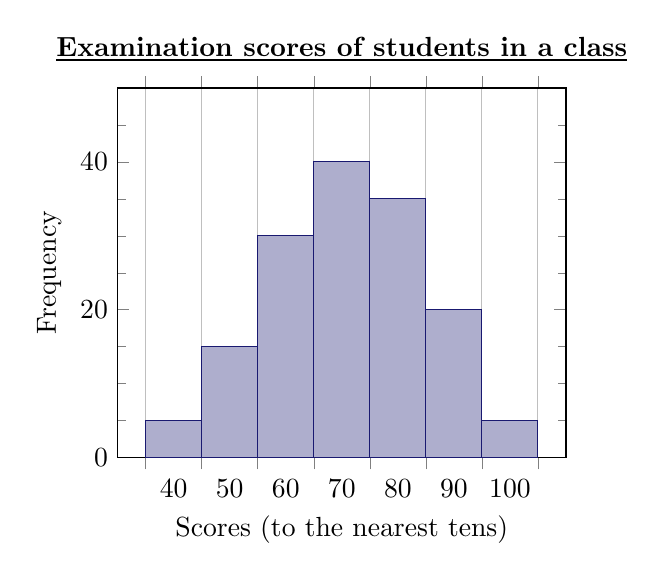
\begin{tikzpicture}
        \begin{axis}[
            width=0.6\textwidth,
            title={\textbf{\underline{Examination scores of students in a class}}},
            xlabel={Scores (to the nearest tens)},
            ylabel={Frequency},
            xmin=35, xmax=115,
            ymin=0, ymax=50,
            xtick distance=10,
            minor y tick num = 3,
            ybar interval
        ]

        \addplot+[ybar interval, fill=MidnightBlue!35, draw=MidnightBlue] plot coordinates { (40, 5) (50, 15) (60, 30) (70, 40) (80, 35) (90, 20) (100, 5) (110, 0)};
        
        \end{axis}
    \end{tikzpicture}

    \caption{A histogram.}
    \label{fig:Ch10-histogram}
\end{figure}

This means that we can measure the proportion of our population corresponding to a certain range of values by simply adding up the surface areas.

A continuous variable can be better represented by a \textit{density plot}, where a smooth curve is used instead of discrete bars. The same rule of surface areas representing densities applies.



\subsection{Mean, median, standard deviation and standard score}

\subsubsection{Mean}

Consider a dataset \(\{x_1,\; x_2,\; x_3,\; \cdots,\; x_N\}\) of size \(N\). We define its \textit{mean} or \textit{average} as
%
\begin{align*}
    \mu &= \frac{\text{sum of all values}}{\text{number of values}}\\
    &= \frac{x_1 + x_2 + x_3 + \cdots + x_N}{N} \text{.}
\end{align*}
%
For example, for the dataset of examination scores shown above, the mean is
%
\begin{align*}
    \mu &= \frac{\text{total score across students}}{\text{number of students}}\\
    &= \frac{40 \times 5 + 50 \times 15 + 60 \times 30 + 70 \times 40 + 80 \times 35 + 90 \times 20 + 100 \times 5}{5 + 15 + 30 + 40 + 35 + 20 + 5}\\
    &= \frac{10650}{150}\\
    &= 71\text{.}
\end{align*}

Note that the average, when used as a descriptor to represent the dataset, can sometimes be misleading as it is sensitive to extreme values. For example, it might be technically correct to say that
%
\begin{quote}
    \textit{``Diaper users have an approximate average age of 25 years old.''}
\end{quote}
%
even though that's not very informative or useful.



\subsubsection{Median}

A different descriptor is called the \textit{median}, which is defined as the number \(v\) such that \(50\%\) of the values are smaller than or equal to \(v\) (while the other \(50\%\) are greater than or equal to \(v\)). This means that given a sorted dataset:
%
\begin{itemize}
    \item If the number of values in the dataset is odd, the median is the value in the middle; whereas
    \item If the number of values in the dataset is even, the median is the average of the two central values.
\end{itemize}
%
For the dataset above, the median is \(v = 70\).



\subsubsection{Standard deviation}

Furthermore, we define the standard deviation of a dataset, denoted as \(\sigma\) or SD, as follows.
%
\[\sigma = \sqrt{\frac{(x_1 - \mu)^2 + (x_2 - \mu)^2 + (x_3 - \mu)^2 + \cdots + (x_N - \mu)^2}{N}}\]
%
This describes the disperson of values around the mean. The dataset above has a standard deviation of approximately \(13.988\).



\subsubsection{\textit{Z}-value (Standard score)}

Lastly, given a value in a dataset, its \textit{\(z\)-value} or \textit{standard score} is defined as the number of standard deviations by which it is above or below the dataset's mean.
%
\[z = \frac{x - \mu}{\sigma}\]
%
See figure \ref{fig:Ch10-z-value}.

\begin{figure}[H]
    \centering

    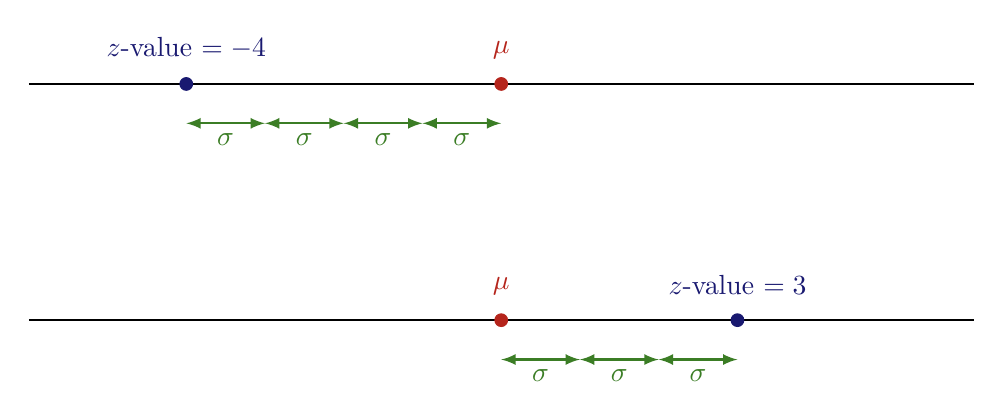
\begin{tikzpicture}[scale=1]
        \draw[thick] (-6,0)--(6,0);

        \filldraw[BrickRed] (0, 0) circle [radius=0.08] node[above, shift={(0, 0.2)}] {\(\mu\)};

        \filldraw[MidnightBlue] (-4, 0) circle [radius=0.08] node[above, shift={(0, 0.2)}] {\(z\)-value \(= -4\)};

        \foreach \i in {-4,...,-1} {
            \draw[OliveGreen, thick, <->, >=latex] (\i,-0.5)--(\i+1,-0.5) node[below, pos=0.5] {\(\sigma\)};
        }

        \begin{scope}[shift={(0, -3)}]
            \draw[thick] (-6,0)--(6,0);

            \filldraw[BrickRed] (0, 0) circle [radius=0.08] node[above, shift={(0, 0.2)}] {\(\mu\)};

            \filldraw[MidnightBlue] (3, 0) circle [radius=0.08] node[above, shift={(0, 0.2)}] {\(z\)-value \(= 3\)};

            \foreach \i in {0,1,2} {
                \draw[OliveGreen, thick, <->, >=latex] (\i,-0.5)--(\i+1,-0.5) node[below, pos=0.5] {\(\sigma\)};
            }
        \end{scope}
    \end{tikzpicture}
    
    \caption{The \(z\)-value is defined as the number of standard deviations by which an element of a dataset is above or below the dataset's mean. Elements lower than the mean are given negative \(z\)-values while those higher than the mean are given positive \(z\)-values.}
    \label{fig:Ch10-z-value}
\end{figure}


\subsection{Normal distribution}

Many real-life phenomena show a density pattern known as the \textit{normal distribution}, which was introduced in the previous section. This results in a histogram with a shape known as the \textit{bell curve}.

\begin{figure}[H]
    \centering

    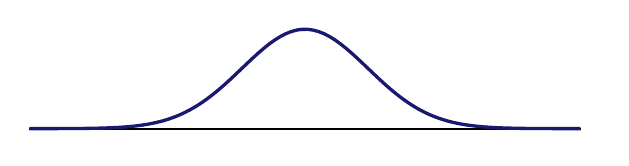
\begin{tikzpicture}[scale=2]
        \draw[thick] (-1.75,0)--(1.75,0);

        \def\sd{0.4};
        \def\mean{0};

        \draw [MidnightBlue, very thick, domain=-1.75:1.75, samples=100] plot (\x,{exp(-0.5*((\x-\mean)/\sd)^2)/sqrt(6.28*\sd)}) node[right, MidnightBlue] {};

    \end{tikzpicture}
    
    \caption{Graphing a normal distribution gives a bell curve.}
    \label{fig:Ch10-bell-curve}
\end{figure}

As shown in figure \ref{fig:Ch10-normal-distribution-and-SDs}, the normal distribution has the following properties:
%
\begin{itemize}
    \item The values within one standard deviation of the mean account for roughly \(68\%\) of the set.
    \item The values within two standard deviations of the mean account for about \(95\%\) of the set.
    \item The values within three standard deviations of the mean account for about \(99.7\%\) of the set.
\end{itemize}

\begin{figure}[H]
    \centering
    \includegraphics[width=0.6\textwidth]{Images/NormalDistAndSDs.png}
    \caption{The normal distribution and its standard deviation.}
    \label{fig:Ch10-normal-distribution-and-SDs}
\end{figure}

The prevalence of the normal distribution in real-world data means that we can often assume that a large enough dataset must follow such a distribution.



\subsection{Standardising a normal distribution}

As we've seen before, a normal distribution can take many forms as it is parameterised by the mean \(\mu\) and the standard deviation \(\sigma\). \textit{Standardisation} refers to the process of transforming any general normal distribution into a \textit{standardised} normal distribution, where \(\mu = 0\) and \(\sigma = 1\).

\begin{figure}[H]
    \centering

    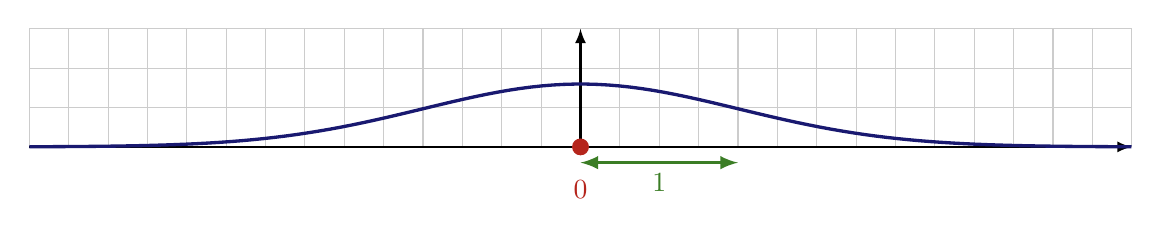
\begin{tikzpicture}[scale=2]
        \draw[thin,gray!40, step=0.25] (-3.5,0) grid (3.5, 0.75);
        \draw[thick, ->, >=latex] (-3.5,0)--(3.5,0);
        \draw[thick, ->, >=latex] (0,0)--(0,0.75);

        \def\sd{1};
        \def\mean{0};

        \draw [MidnightBlue, very thick, domain=-3.5:3.5, samples=100] plot (\x,{exp(-0.5*((\x-\mean)/\sd)^2)/sqrt(6.28*\sd)});

        \draw[OliveGreen, very thick, <->, >=latex, shift={(0,-0.1)}] (0,0)--(\sd,0) node[below, pos=0.5] {\(\sd\)};

        \filldraw[BrickRed] (0, 0) circle [radius=0.05] node[below, shift={(0, -0.3)}] {\(\mean\)};
    \end{tikzpicture}
    
    \caption{A standardised normal distribution. This distribution has \(\mu = 0\) and \(\sigma = 1\).}
    \label{fig:Ch10-standardised-normal-dist}
\end{figure}

Suppose a random variable \(X\) has a normal distribution with a mean (or expected value) of \(\mu\) and a standard deviation of \(\sigma\). In the diagrams that follow, we will take the values \(\mu = 2\) and \(\sigma = 0.3\).

\begin{figure}[H]
    \centering

    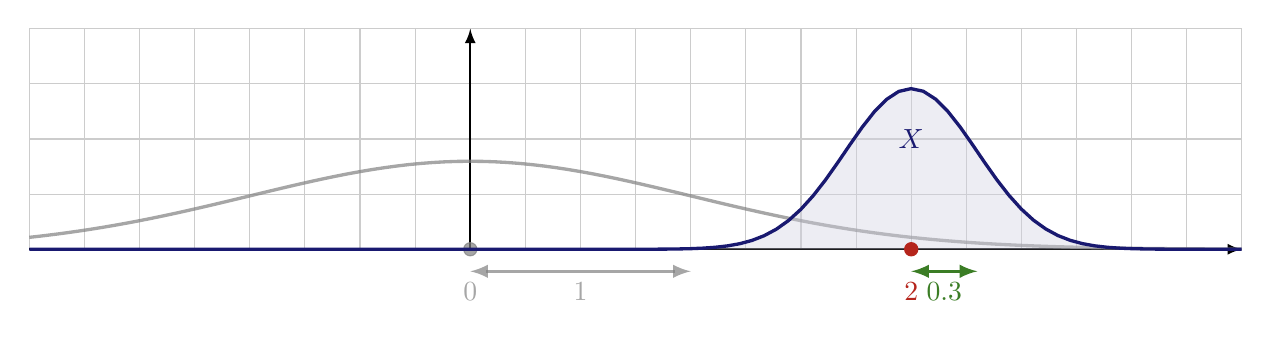
\begin{tikzpicture}[scale=2.8]
        \draw[thin,gray!40, step=0.25] (-2,0) grid (3.5, 1);
        \draw[thick, ->, >=latex] (-2,0)--(3.5,0);
        \draw[thick, ->, >=latex] (0,0)--(0,1);


        \def\sd{1};
        \def\mean{0};

        \draw [gray, opacity=0.7, very thick, domain=-2:3.5, samples=100] plot (\x,{exp(-0.5*((\x-\mean)/\sd)^2)/sqrt(6.28*\sd)});

        \draw[gray, opacity=0.7, very thick, <->, >=latex, shift={(0,-0.1)}] (\mean,0)--(\mean+\sd,0) node[below, pos=0.5] {\(\sd\)};

        \filldraw[gray, opacity=0.7] (\mean, 0) circle [radius=0.03] node[below, shift={(0, -0.3)}] {\(\mean\)};


        \def\sd{0.3};
        \def\mean{2};

        \draw [MidnightBlue, fill=MidnightBlue!20, fill opacity=0.4, very thick, domain=-2:3.5, samples=100] plot (\x,{exp(-0.5*((\x-\mean)/\sd)^2)/sqrt(6.28*\sd)});

        \draw[OliveGreen, very thick, <->, >=latex, shift={(0,-0.1)}] (\mean,0)--(\mean+\sd,0) node[below, pos=0.5] {\(\sd\)};

        \filldraw[BrickRed] (\mean, 0) circle [radius=0.03] node[below, shift={(0, -0.3)}] {\(\mean\)};

        \node[MidnightBlue] at (\mean,0.5) {\(X\)};
    \end{tikzpicture}
    
    \caption{A random variable \(X\) has a normal distribution where \(\mu = E(X) = 2\) and \(\sigma = 0.3\). The standardised normal distribution is shown in grey.}
    \label{fig:Ch10-general-normal-dist}
\end{figure}

To transform this curve into the grey one, we can start by subtracting \(\mu\) from \(X\). This results in a new random variable \(Y = X - \mu\) of the same standard deviation and whose bell curve is centered at the origin. This is verified mathematically by the following claim.

\begin{quote}
    \textbf{Claim.} Consider a random variable \(X\) with mean \(\mu\). For any constant \(a\), the random variable given by \(Y = X - a\) must have a mean of \(\mu - a\). Both \(X\) and \(Y\) have the same standard deviation \(\sigma\).

    \textbf{Proof.} For the mean, we have
    %
    \begin{align*}
        E(Y) &= E(X - a)\\
        &= E(X) - E(a)\\
        &= E(X) - a\\
        &= \mu - a\text{.}
    \end{align*}
    %
    For the standard deviation, we consider the variance of both variables.
    %
    \begin{align*}
        \text{Variance of } Y &= E((Y - E(Y))^2)\\
        &= E((Y - (\mu - a))^2) \tag{proved earlier}\\
        &= E((X - a - (\mu - a))^2)\\
        &= E((X - \mu)^2)\\
        &= E((X - E(X))^2)\\
        &= \text{Variance of } X 
    \end{align*}
    %
    Since their variances are identical, they must share the same standard deviation.
\end{quote}


\begin{figure}[H]
    \centering

    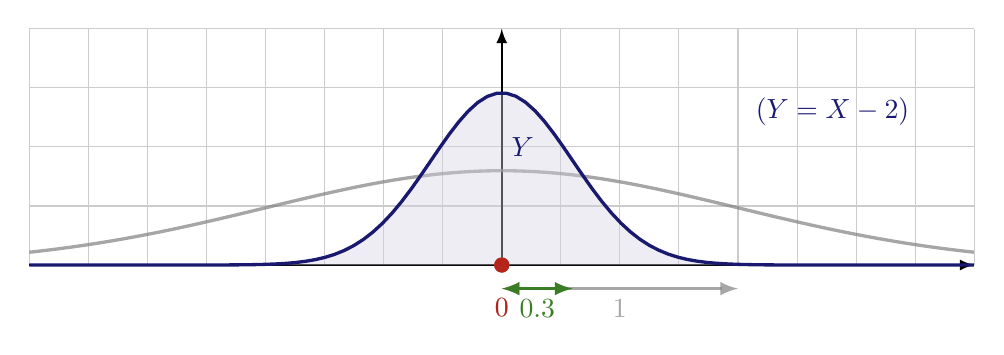
\begin{tikzpicture}[scale=3]
        \draw[thin,gray!40, step=0.25] (-2,0) grid (2, 1);
        \draw[thick, ->, >=latex] (-2,0)--(2,0);
        \draw[thick, ->, >=latex] (0,0)--(0,1);


        \def\sd{1};
        \def\mean{0};

        \draw [gray, opacity=0.7, very thick, domain=-2:2, samples=100] plot (\x,{exp(-0.5*((\x-\mean)/\sd)^2)/sqrt(6.28*\sd)});

        \draw[gray, opacity=0.7, very thick, <->, >=latex, shift={(0,-0.1)}] (\mean,0)--(\mean+\sd,0) node[below, pos=0.5] {\(\sd\)};

        \filldraw[gray, opacity=0.7] (\mean, 0) circle [radius=0.03] node[below, shift={(0, -0.3)}] {\(\mean\)};


        \def\sd{0.3};
        \def\mean{0};

        \draw [MidnightBlue, fill=MidnightBlue!20, fill opacity=0.4, very thick, domain=-2:2, samples=100] plot (\x,{exp(-0.5*((\x-\mean)/\sd)^2)/sqrt(6.28*\sd)});

        \draw[OliveGreen, very thick, <->, >=latex, shift={(0,-0.1)}] (\mean,0)--(\mean+\sd,0) node[below, pos=0.5] {\(\sd\)};

        \filldraw[BrickRed] (\mean, 0) circle [radius=0.03] node[below, shift={(0, -0.3)}] {\(\mean\)};

        \node[MidnightBlue, right] at (\mean,0.5) {\(Y\)};

        \node[MidnightBlue] at (1.4,0.65) {\((Y = X - 2)\)};
    \end{tikzpicture}
    
    \caption{Subtract \(\mu\) from \(X\) to create a new random variable \(Y\) with a centered bell curve.}
    \label{fig:Ch10-centered-normal-dist}
\end{figure}


Next, we want to modify \(Y\)'s bell curve such that its standard deviation \(\sigma\) equals \(1\). To do this, we divide \(Y\) by \(\sigma\), resulting in a new random variable \(Z = Y / \sigma\). Note that this means that \(Z\) has a standardised distribution. This is once again supported by the following claim.

\begin{quote}
    \textbf{Claim.} Consider a random variable \(X\) with mean \(\mu\) and standard deviation \(\sigma\). For any constant \(b\), the random variable given by \(Y = bX\) must have a mean of \(b\mu\) and a standard deviation of \(b\sigma\).

    \textbf{Proof.} For the mean, we have
    %
    \begin{align*}
        E(Y) &= E(bX)\\
        &= \sum_{x \;\in\; \text{possible values of \(X\)}} (bx \times P(bX = bx))\\
        &= \sum_{x \;\in\; \text{possible values of \(X\)}} (bx \times P(X = x))\\
        &= b \times \left( \sum_{x \;\in\; \text{possible values of \(X\)}} (x \times P(X = x))\right)\\
        &= b E(X)
    \end{align*}
    %
    For the standard deviation, we consider the variance of both variables.
    %
    \begin{align*}
        \text{Variance of } Y &= E(Y^2) - E(Y)^2\\
        &= E(Y^2) - (b E(X))^2 \tag{proved earlier}\\
        &= E(b^2 X^2) - b^2 (E(X))^2\\
        &= b^2 E(X^2) - b^2 (E(X))^2\\
        &= b^2 (E(X^2) - (E(X))^2)\\
        &= b^2 (\text{Variance of } X)
    \end{align*}
    %
    This means that the standard deviation of \(Y\) is \(b\) times that of \(X\).
\end{quote}

This means that any random variable \(X\) with a normal distribution can be standardised as
%
\[Z = \frac{Y}{\sigma} = \frac{X - \mu}{\sigma}\text{.}\]

\begin{figure}[H]
    \centering

    \begin{tikzpicture}[scale=2.5]
        \draw[thin,gray!40, step=0.25] (-3,0) grid (3, 1);
        \draw[thick, ->, >=latex] (-3,0)--(3,0);
        \draw[thick, ->, >=latex] (0,0)--(0,1);

        \def\sd{1};
        \def\mean{0};

        \draw [MidnightBlue, fill=MidnightBlue!20, fill opacity=0.4, very thick, domain=-3:3, samples=100] plot (\x,{exp(-0.5*((\x-\mean)/\sd)^2)/sqrt(6.28*\sd)});

        \draw[OliveGreen, very thick, <->, >=latex, shift={(0,-0.1)}] (\mean,0)--(\mean+\sd,0) node[below, pos=0.5] {\(\sd\)};

        \filldraw[BrickRed] (\mean, 0) circle [radius=0.03] node[below, shift={(0, -0.3)}] {\(\mean\)};

        \node[MidnightBlue, right] at (\mean,0.25) {\(Z\)};

        \node[MidnightBlue] at (1.4,0.6) {\(\left(Z = \dfrac{X-\mu}{\sigma}\right)\)};
    \end{tikzpicture}
    
    \caption{A standardised normal distribution.}
    \label{fig:Ch10-standardisation-complete}
\end{figure}


\subsection{Sampling and confidence intervals}

\subsubsection{What is sampling?}

In real life, examining every member of a population is not always possible. Instead, we often resort to \textit{sampling}, where we infer properties of the entire population by examining a small subset of it. This raises the question: How can we make sure that are sample is trustworthy?

In general, a sample is more trustworthy if:
%
\begin{itemize}
    \item It has a larger size.
    \item It is taken as randomly (i.e. without bias) as possible.
\end{itemize}

To quantify the trustworthiness of a sample, we introduce the concept of a \textit{confidence interval}.



\subsubsection{What is a confidence interval?}

Assume that the variable under study is normally distributed. Here we will once again use students' examination scores as an example.

Suppose we don't know the true value of the mean score, and we want to estimate this mean using the following sample of size \(n = 5\).
%
\[\text{Sample} = \{40, 50, 80, 80, 90\}\]
%
This gives us an estimated mean score of
%
\[\mu_n = \frac{40 + 50 + 80 + 90 + 90}{5}
= 68\text{.}\]
%
Based on this information alone:
%
\begin{itemize}
    \item It is highly likely that the true mean is somewhere around \(68\). For example, the true mean is probably something like \(66\), \(67\) or \(70\).

    \item It is however unlikely that the true mean is extremely far away from the true mean. For example, we are almost certain that the true mean is not going to be something like \(14\) or \(98\).
\end{itemize}

To formalise this reasoning, we may say that something like
%
\begin{quote}
    Given an estimated mean of \(\mu_n = 68\), the true mean has a \(95\%\) probability of being inside the interval \([49,\; 87]\).
\end{quote}
%
This interval is called the \textit{confidence interval}, which changes depending on the specified confidence level (\(95\%\) in this case). This raises the question: How can we find a confidence interval given a sample and a confidence level?




\subsubsection{How to compute confidence intervals}

Given a confidence level \(r\%\), we want to find the critical \(z\)-value that captures the central \(r\%\) of the normal distribution. For example, for a confidence level of \(95\%\), the corresponding critical \(z\) value is \(1.96\). This conversion can be done computationally or via a table.

\begin{figure}[H]
    \centering

    \begin{tikzpicture}[scale=5]
        \draw[thin,gray!40, step=0.25] (-1.5,0) grid (1.5, 0.75);
        \draw[thick, ->, >=latex] (-1.5,0)--(1.5,0);
        \draw[thick, ->, >=latex] (0,0)--(0,0.75);

        \def\sd{0.4};
        \def\mean{0};
        \def\critX{1.96*\sd};

        \coordinate (CurveLeftEdge) at (-\critX, {exp(-0.5*((-\critX-\mean)/\sd)^2)/sqrt(6.28*\sd)});
        \coordinate (CurveRightEdge) at (\critX, {exp(-0.5*((\critX-\mean)/\sd)^2)/sqrt(6.28*\sd)});

        \filldraw [OliveGreen!15, opacity=0.6, very thick, domain=-\critX:\critX, samples=100] plot (\x,{exp(-0.5*((\x-\mean)/\sd)^2)/sqrt(6.28*\sd)}) node[right, MidnightBlue] {};
        \filldraw [OliveGreen!15, opacity=0.6] (-\critX, 0) rectangle (CurveRightEdge);

        \draw[OliveGreen, very thick, dashed] (-\critX, 0) -- (CurveLeftEdge);
        \draw[OliveGreen, very thick, dashed] (\critX, 0) -- (CurveRightEdge);

        \draw [MidnightBlue, very thick, domain=-1.5:1.5, samples=100] plot (\x,{exp(-0.5*((\x-\mean)/\sd)^2)/sqrt(6.28*\sd)}) node[right, MidnightBlue] {};
        

        \draw[BurntOrange, very thick, <->, >=latex] (-\critX,0)--(-\sd,0) node[above, pos=0.5] {\(0.96\sigma\)};
        \draw[BurntOrange, very thick, <->, >=latex] (-\sd,0)--(0,0) node[above, pos=0.5] {\(\sigma\)};
        \draw[BurntOrange, very thick, <->, >=latex] (0,0)--(\sd,0) node[above, pos=0.5] {\(\sigma\)};
        \draw[BurntOrange, very thick, <->, >=latex] (\sd,0)--(\critX,0) node[above, pos=0.5] {\(0.96\sigma\)};

        \filldraw[BrickRed] (0, 0) circle [radius=0.02] node[below, shift={(0, -0.3)}] {\(\mu\)};

        \filldraw[OliveGreen] (\critX, 0) circle [radius=0.015] node[below, shift={(0, -0.3)}, text width=1.5cm, align=center] {\(z\)-value \(1.96\)};

        \filldraw[OliveGreen] (-\critX, 0) circle [radius=0.015] node[below, shift={(0, -0.3)}, text width=1.5cm, align=center] {\(z\)-value \(1.96\)};

        \draw [decorate, decoration={calligraphic brace, amplitude=5pt}, pen colour=OliveGreen, ultra thick] (-\critX, 0.8) --  (\critX, 0.8) node[above=5pt, pos=0.5] {\large \color{OliveGreen} \(\mathbf{95\%}\)};

        \draw [decorate, decoration={calligraphic brace, amplitude=5pt}, pen colour=BrickRed!60, ultra thick] (-1.5, 0.8) --  (-\critX, 0.8) node[above=5pt, pos=0.5] {\large \color{BrickRed!60} \(\mathbf{2.5\%}\)};

        \draw [decorate, decoration={calligraphic brace, amplitude=5pt}, pen colour=BrickRed!60, ultra thick] (\critX, 0.8) --  (1.5, 0.8) node[above=5pt, pos=0.5] {\large \color{BrickRed!60} \(\mathbf{2.5\%}\)};
    \end{tikzpicture}
    
    \caption{A confidence level of \(95\%\) corresponds to a critical \(z\)-value of \(1.96\).}
    \label{fig:Ch10-critical-z-value}
\end{figure}

Then, we will use the following formula to compute the confidence interval:
%
\[
    \text{Confidence interval} = \left[
        \mu_n - z\left(\frac{\sigma_n}{\sqrt{n}}\right),\;
        \mu_n + z\left(\frac{\sigma_n}{\sqrt{n}}\right)
    \right]
\]
%
where
%
\begin{itemize}
    \item \(\mu_n\) is the mean estimated from the sample.
    \item \(z\) is the critical \(z\)-value that corresponds to the given confidence level.
    \item \(\sigma_n\) is the standard deviation of the sample.
    \item \(n\) is the size of the sample.
\end{itemize}

Using our example from before, we have
%
\begin{align*}
    \text{Confidence interval} &= \left[
        \mu_n - z\left(\frac{\sigma_n}{\sqrt{n}}\right),\;
        \mu_n + z\left(\frac{\sigma_n}{\sqrt{n}}\right)
    \right]\\
    &= \left[
        68 - 1.96\left(\frac{21.679}{\sqrt{5}}\right),\;
        68 + z\left(\frac{21.679}{\sqrt{5}}\right)
    \right]\\
    &= [49.0,\; 87.0]\text{.}
\end{align*}

Hence, we can be \(95\%\) sure that the average examination score of the class lies within the interval \([49.0,\; 87.0]\).



\subsubsection{Derivation of the confidence interval formula}

Here we derive the aforementioned formula for a confidence interval.

Notice that the sample mean \(\mu_n\) is a random variable with a normal distribution. By the central limit theorem\footnote{The central limit theorem is out of the scope of this module. For now, we will take these values as granted.}, this distribution has a mean of \(\mu\) and a variance of \(\sigma^2 / n\). This means that its standard deviation is \(\sigma / \sqrt{n}\).

\begin{figure}[H]
    \centering

    \begin{tikzpicture}[scale=2.8]
        \draw[thin,gray!40, step=0.25] (-2,0) grid (3.5, 1);
        \draw[thick, ->, >=latex] (-2,0)--(3.5,0);
        \draw[thick, ->, >=latex] (0,0)--(0,1);


        \def\sd{1};
        \def\mean{0};

        \draw [gray, opacity=0.7, very thick, domain=-2:3.5, samples=100] plot (\x,{exp(-0.5*((\x-\mean)/\sd)^2)/sqrt(6.28*\sd)});

        \draw[gray, opacity=0.7, very thick, <->, >=latex, shift={(0,-0.1)}] (\mean,0)--(\mean+\sd,0) node[below, pos=0.5] {\(\sd\)};

        \filldraw[gray, opacity=0.7] (\mean, 0) circle [radius=0.03] node[below, shift={(0, -0.3)}] {\(\mean\)};


        \def\sd{0.3};
        \def\mean{2};

        \draw [MidnightBlue, fill=MidnightBlue!20, fill opacity=0.4, very thick, domain=-2:3.5, samples=100] plot (\x,{exp(-0.5*((\x-\mean)/\sd)^2)/sqrt(6.28*\sd)});

        \draw[OliveGreen, very thick, <->, >=latex, shift={(0,-0.1)}] (\mean,0)--(\mean+\sd,0) node[below, pos=0.5] {\(\dfrac{\sigma}{\sqrt{n}}\)};

        \filldraw[BrickRed] (\mean, 0) circle [radius=0.03] node[below, shift={(0, -0.3)}] {\(\mu\)};

        \node[MidnightBlue] at (\mean,0.5) {\(\mu_n\)};
    \end{tikzpicture}
    
    \caption{The sample mean \(\mu_n\) has a normal distribution with mean \(\mu\) and standard deviation \(\sigma/\sqrt{n}\).}
    \label{fig:Ch10-sample-mean-normal-dist}
\end{figure}

We standardise this to get
%
\[\frac{(\mu_n - \mu)\sqrt{n}}{\sigma}\]
%
which has mean \(0\) and standard deviation \(1\). See figure \ref{fig:Ch10-standardised-sample-mean}.

\begin{figure}[H]
    \centering

    \begin{tikzpicture}[scale=2.5]
        \draw[thin,gray!40, step=0.25] (-3,0) grid (3, 1);
        \draw[thick, ->, >=latex] (-3,0)--(3,0);
        \draw[thick, ->, >=latex] (0,0)--(0,1);

        \def\sd{1};
        \def\mean{0};

        \draw [MidnightBlue, fill=MidnightBlue!20, fill opacity=0.4, very thick, domain=-3:3, samples=100] plot (\x,{exp(-0.5*((\x-\mean)/\sd)^2)/sqrt(6.28*\sd)});

        \draw[OliveGreen, very thick, <->, >=latex, shift={(0,-0.1)}] (\mean,0)--(\mean+\sd,0) node[below, pos=0.5] {\(\sd\)};

        \filldraw[BrickRed] (\mean, 0) circle [radius=0.03] node[below, shift={(0, -0.3)}] {\(\mean\)};

        \node[MidnightBlue, right] at (\mean,0.65) {\(\dfrac{(\mu_n - \mu)\sqrt{n}}{\sigma}\)};
    \end{tikzpicture}
    
    \caption{Standardising \(\mu_n\).}
    \label{fig:Ch10-standardised-sample-mean}
\end{figure}

We know from before that in a standardised normal distribution, a critical \(z\)-value of \(1.96\) captures \(95\%\) of the area under the bell curve. In other words, there is a \(95\%\) probability that:
%
\begin{alignat*}{5}
    -1.96 &\leq \frac{(\mu_n - \mu)\sqrt{n}}{\sigma} &&\leq 1.96\\
    -1.96\sigma &\leq (\mu_n - \mu)\sqrt{n} &&\leq 1.96\sigma\\
    \frac{-1.96\sigma}{\sqrt{n}} &\leq \hspace{1.5em}\mu_n - \mu &&\leq \frac{1.96\sigma}{\sqrt{n}}\\
    \mu_n + \frac{1.96\sigma}{\sqrt{n}} &\geq \hspace{2.25em}\mu &&\geq \mu_n - \frac{1.96\sigma}{\sqrt{n}}
\end{alignat*}
%
which can be generalised to give
%
\[\mu_n + z\left(\frac{\sigma}{\sqrt{n}}\right) \geq \mu \geq \mu_n - z\left(\frac{\sigma}{\sqrt{n}}\right)\text{.}\]
%
Assuming \(\sigma_n \approx \sigma\) gives
%
\[\mu_n + z\left(\frac{\sigma_n}{\sqrt{n}}\right) \geq \mu \geq \mu_n - z\left(\frac{\sigma_n}{\sqrt{n}}\right)\]
%
which yields the formula for the confidence interval.



\subsection{Hypothesis testing}

Suppose we have a coin. We toss the coin 20 times, and the result consists of 15 heads. Is the coin biased towards heads?

\begin{figure}[H]
    \centering

    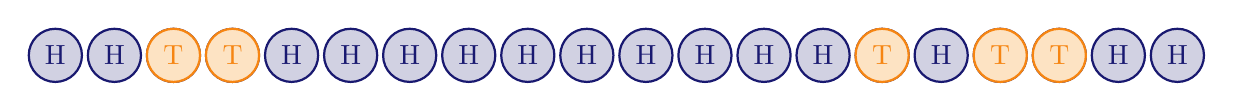
\begin{tikzpicture}[scale=0.75]
        \foreach \x in {0,...,19} {
            \draw[thick, MidnightBlue, fill=MidnightBlue!20] (\x,0) circle [radius=0.45] node {H};
        }
        \foreach \x in {2, 3, 14, 16, 17} {
            \draw[thick, BurntOrange, fill=BurntOrange!20] (\x,0) circle [radius=0.45] node {T};
        }
    \end{tikzpicture}
    
    \caption{Is the coin biased?}
    \label{fig:Ch10-is-coin-biased}
\end{figure}

At first glance, we may be tempted to say yes --- the coin is indeed biased towards heads. However, the result of tossing 15 out of 20 heads remains entirely plausible even with a completely fair coin.

To tackle this conundrum, we can utilise the idea of \textit{hypothesis testing}.

For starters, we state the following hypotheses:
%
\begin{itemize}
    \item \textbf{Null hypothesis (H0).} ``The coin is fair.''
    \item \textbf{Alternative hypothesis (H1).} ``The coin is biased towards heads.''
\end{itemize}
%
The \textit{null hypothesis}, denoted as H0, refers to the ``default'' situation. On the contrary, the \textit{alternative hypothesis}, denoted as H1, refers to the phenomenon that is suspected to be true.

We then decide on a \textit{significance threshold} --- the probability of an event that we consider too unlikely to happen only by chance. For this example, we will set the significance threshold to \(5\%\).

Next, we calculate the \textit{\(p\)-value}, which is the probability that results at least as extreme as ours happens, assuming that the null hypothesis is verified. In the coin-tossing example, we want to evaluate
%
\[P(\text{at least 15 out of 20 heads} \;\vert\; \text{H0})\]
%
as the \(p\)-value. We calculate this as
%
\begin{align*}
    p \text{-value} &= P(X \geq 15 \;\vert\; \text{H0})\\
    &= P(X = 15 \;\vert\; \text{H0}) + P(X = 16 \;\vert\; \text{H0}) + \cdots + P(X = 20 \;\vert\; \text{H0})\\
    &= \left(\frac{1}{2}\right)^{20} {20 \choose 15} + \left(\frac{1}{2}\right)^{20} {20 \choose 16} + \cdots + \left(\frac{1}{2}\right)^{20} {20 \choose 20}\\
    &\approx 0.021\\
    &= 2.1\%
\end{align*}
%
which is smaller than the significance threshold of \(5\%\). This means that getting 15 heads out of 20 coin tosses is far too unlikely for the coin to be fair. Hence, our test is considered \textit{significant} and we reject the null hypothesis H0.

Note that in the opposite scenario where the \(p\)-value exceeds the significance threshold, we \textit{cannot} say we ``accept the alternative hypothesis''. Instead, we must say that we have failed to reject H0, and that no conclusion can be reached.